\section{Singleton Pattern}

Singleton pattern is one of the simplest design patterns in Java. This type of design pattern comes under creational pattern as this pattern provides one of the best ways to create an object. This pattern involves a single class which is responsible to create an object while making sure that only single object gets created.

\subsection{Class Diagram}

\begin{figure}[h]
\centering
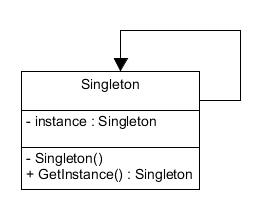
\includegraphics[scale=0.5]{singleton}
\caption{Class Diagram of Singleton Pattern}
\end{figure}

\newpage
\subsection{Source Code (Java)}

\subsubsection{OS Class as Singleton}

\begin{minted}{java}
package singleton;

/* OS as singleton class. */

class OS {
    /* 1. Create a static object. */
    static OS obj = new OS();
    int value = 10;


    /* 2. The user shouldn't be able to 
    create instance through constructor. */
    private OS() {
    }

    /* 3. Static method to return object 
    which also return static object. */
    public static OS getInstance() {
        return obj;
    }

    /* 4. (Optional) Create a method to 
    alter the value(value) so that we can
    observer the instance being shared
    among every objects.*/
    public void setValue(int value){
        this.value = value;
    }
}
\end{minted}

\subsubsection{Driver Class}

\begin{minted}{java}
package singleton;

/* Class to demonstrate singleton behaviour of OS class. */

public class Singleton {
    public static void main(String[] args) {
        OS obj1 = OS.getInstance();
        OS obj2 = OS.getInstance();

        System.out.println(obj1.value);
        System.out.println(obj2.value);

        /* Changing the value property of obj1 object
        will also change the value property of obj2
        object. It happens because the instance is shared
        between every objects.
         */
        obj1.setValue(20);

        System.out.println(obj1.value);
        System.out.println(obj2.value);
    }
}
\end{minted}

\subsection{Output}

\begin{minted}{text}
10
10

20
20
\end{minted}